\documentclass[phd]{byuprop}
% Options for this class include the following (* indicates default):
%
%   10pt -- 10 point font size
%   11pt -- 11 point font size
%   12pt (*) -- 12 point font size
%
%   ms -- produce a thesis proposal (off)
%   areaexam -- produce a research area overview (off)
%   phd -- produce a dissertation proposal (off)
%
%   singlespacing -- single-spaced lines
%   doublespacing -- double-spaced lines
%
%   layout -- show layout lines on the pages, helps with overfull boxes (off)
%   grid -- show a half-inch grid on every page, helps with printing (off)


% This command fixes my particular printer, which starts 0.03 inches too low,
% shifting the whole page down by that amount.  This shifts the document
% content up so that it comes out right when printed.
%
% Discovering this sort of behavior is best done by specifying the ``grid''
% option in the class parameters above.  It prints a 1/2 inch grid on every
% page.  You can then use a ruler to determine exactly what the printer is
% doing.
%
% Uncomment to shift content up (accounting for printer problems)
%\setlength{\voffset}{-.03in}

% Here we set things up for invisible hyperlinks in the document.  This makes
% the electronic version clickable without changing the way that the document
% prints.  It's useful, but optional.  Note that if you use latex instead of
% pdflatex, you should change "pdftex" to "ps2pdf".
\usepackage[
    pdftex,
    bookmarks=true,
    breaklinks=true,
    raiselinks=true,
    pdfborder={0 0 0},
    colorlinks=false,
    ]{hyperref}
    
\usepackage{caption}
\usepackage{subcaption}
\usepackage{bm}
\usepackage{amsfonts}
\usepackage{amsmath}
\usepackage{comment}

\usepackage{amsthm}
\usepackage{multirow}
\usepackage{pbox}

\newtheorem{mylem}{Lemma}
\newtheorem{myhyp}{Assumption}
\newtheorem{myprop}{Property}
\newtheorem{mythm}{Theorem}
\newtheorem{mydef}{Definition}

% Rewrite the itemize, description, and enumerate environments to have more
% reasonable spacing:
\newcommand{\ItemSep}{\itemsep 0pt}
\let\oldenum=\enumerate
\renewcommand{\enumerate}{\oldenum \ItemSep}
\let\olditem=\itemize
\renewcommand{\itemize}{\olditem \ItemSep}
\let\olddesc=\description
\renewcommand{\description}{\olddesc \ItemSep}

% Get a little less fussy about word spacing on a line.  Sometimes produces
% ugly results, so keep your eyes peeled.
\sloppy

% Important settings for the byuprop class. %
%%%%%%%%%%%%%%%%%%%%%%%%%%%%%%%%%%%%%%%%%%%%%

% Because I use these things in more than one place, I created new commands for
% them.  I did not use \providecommand because I absolutely want LaTeX to error
% out if these already exist.
\newcommand{\Title}{
From qualitative to quantitative: supporting the robot understanding the human in path planning
}
\newcommand{\Author}{Daqing Yi}
\newcommand{\SubmissionMonth}{April}
\newcommand{\SubmissionYear}{2015}

% Take these from the commands defined above
\title{\Title}
\author{\Author}
\monthsubmitted{\SubmissionMonth}
\yearsubmitted{\SubmissionYear}

% Committee members
\committeechair{Michael~A.~Goodrich}
\committeemembera{Kevin~D.~Seppi}
\committeememberb{Randal~W.~Beard}
\committeememberc{Mark~J.~Clement}
\committeememberd{Parris~K.~Egbert}

% Department graduate coordinator
\graduatecoordinator{Quinn~Snell}

\documentabstract{%
% The proposal abstract should be 1 to 2 paragraphs.
%This document is an example of how to use the byuprop {\LaTeX} class file.  The class creates Ph.D. and Master's documents equally well, producing all appropriate preamble content and adhering precisely to the minimum formatting requirements.

%Note that there is a blank line between paragraphs, here.
Improvements in robot autonomy are changing human-robot interaction from low-level manipulation to high-level task-based collaboration.
When a robot can independently and autonomously execute the tasks, the roles of a human in a human-robot team are a collaborator and a task supervisor.
%How the robot reads the human's qualitative intent into the quantitative model
How the robot understands the human's intent and how the robot responds to environment dynamics and uncertainty determine the collaborative performance and the interaction experience.
In the literature on human-machine interaction, mental models play a key role.
Operationally, a mental model is a representation of how current states are turned into consequences through the actions of an agent.
A human's intent can be operationally defined as a preference over consequences produced by a robot's actions and possibly as a preference over the actions used by the robot to produce a desirable consequence.

We propose a series of robot motion planning algorithms, each of which is designed to support some aspect of a human's intent.
For motion planning, we propose algorithms that support a versatile human intent set.
We consider planning problems: planning with a human-motion constraint, planning with topological requirement, planning with multiple objectives and planning from verbal instruction.
}

%%%%%%%%%%%%%%%%%%%%%%%%%%%%%%%%%%%%%%%%%%%%%

% Set up the internal PDF information so that it becomes part of the document
% metadata.  The pdfinfo command will display this. Be sure to set the document
% type and add your own keywords.
\hypersetup{%
    pdftitle=\Title,%
    pdfauthor=\Author,%
    %pdfsubject={Document Type, BYU CS Department: %
    %            Submitted \SubmissionMonth~\SubmissionYear, Created \today},%
    pdfsubject={PhD Proposal, BYU CS Department: %
                Submitted \SubmissionMonth~\SubmissionYear, Created \today},%
    pdfkeywords={Multi-Objective Optimization, Homotopy class, Path Planning, Human-Robot Collaboration, Particle Swarm Optimization},%
}

% These packages allow the bibliography to be sorted alphabetically and allow references to more than one paper to be sorted and compressed (i.e. instead of [5,2,4,6] you get [2,4-6])
\usepackage[numbers,sort&compress]{natbib}
\usepackage{hyperref}

% Additional packages required for your specific thesis go here. I've left some I use as examples.
\usepackage{graphicx}
\usepackage{pdfsync}

\begin{document}

% Produce the preamble
\maketitle

%%%%%%%%%%%%%%%%%%%%%%%%%%%%%%%%%%%%%%%%%%%%%%%%%%%%%%%%%%%%%%%%%%%%%%%%%%%%%%%
\section{Introduction}
% 1-2 pages
% Answers:
% 1) What problem do you want to solve?
% 2) Who cares about this problem and why?

\subsection{Shared Mental Model in Human-Robot Collaboration}

The ways robots and humans ``think'' are very different.
Humans are experts at making qualitative decisions, from low-level movement to high-level reasoning,
and robots show great strength in solving quantitative problems like high-speed data processing, high-precision repeated motion, etc.
In organizing humans and robots in a team, the differences between humans and robots cannot be ignored.
Due to the difference, humans and robots are often assigned different roles when collaborating in a team.
In teamwide collaboration, there is often a team task, which is defined as the goal of the team.
A team ``coach'' splits the team task into subtasks for the team players.
In the spirit of human-centered intelligence, the team ``coach'' is a human, who executes high-level planning, splits tasks and schedules teammates.
The team players include both humans and robots.
Relatively speaking, humans' strength is high-level decision making, and robots' strength is low-level operations.
Robots can
\begin{itemize}
\item deliver constant and stable performance without fatigue;
\item collect versatile formats of observation data by different sensors; and
\item access some particular spaces that humans cannot reach and etc.
\end{itemize}
Humans can
\begin{itemize}
\item adapt to environment change in task execution;
\item respond to unexpected occurrences that happen accidentally; and
\item be robust to the vague or unmatched information. 
\end{itemize}
  
For example, in a rescue and search task, robots perform dull, dirty and dangerous tasks, and alert a human only when an abnormality is detected.
The human then deals with the abnormal occurrence.
Also robot players can explore some dangerous and inaccessible regions to humans, and assist human players when needed.
Particularly, when there is any situation change, human players will need to organize robot players to react.

In a collaborative team, team functioning is supported by a shared mental~\cite{Jonker:2010:SMM:2018118.2018128}.

The running of the shared mental model is by the information sharing between the agents in the team.
The directions of the information flow are determined by the team roles~\cite{Yen_implementingshared}.
Figure \ref{fig:team_info_flow} gives an example of the information flow in a human-robot team.
In completing the team task, a human coach distributes the subtasks to human players and robot players, which indicates the information flowing toward players.
The {\em offline information flow} brings the priori of the shared mental model to the player, which includes~\cite{Goodrich2013}
\begin{itemize}
\item {\em team task model} : the knowledge of procedures, equipment, situations and constraint; 
\item {\em teammate model} : the knowledge of teammates skills, abilities and tendencies.
\end{itemize}
The offline information flow impacts the effectiveness of task execution.
It guarantees that the player can understand the coach's intent so that the planning and execution of the autonomous agent is for correct rationality.
While the task is being executed, the players also share the information with each other, which forms the mutual information flow between the players.
The {\em online information flow} exchanges the information between team players by interaction, which is about
\begin{itemize} 
\item {\em team interaction model} : knowledge of roles, responsibilities, information sources, communication channels, role interdependencies and task execution states.
\end{itemize}
The online information flow improves the efficiency of task execution.
A better mutual information improves the team performance.

\begin{figure}[hbtp]
\centering
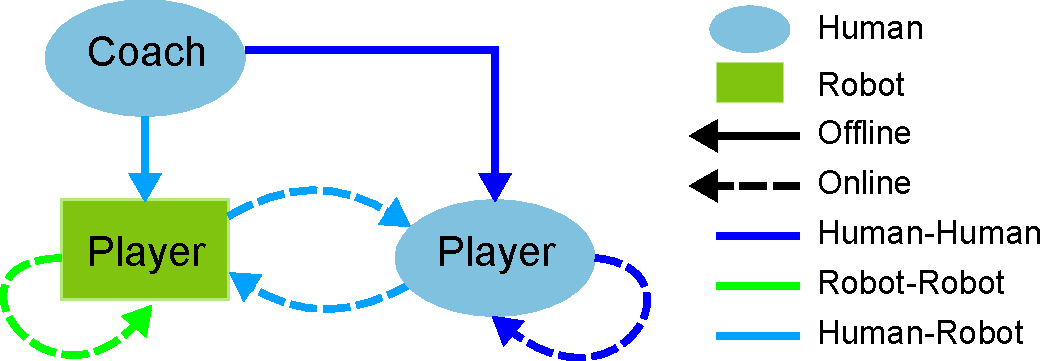
\includegraphics[width=0.6\linewidth]{./fig/team_info_flow.pdf}
\caption{The information flow in the team.}
\label{fig:team_info_flow}
\end{figure}

Due to the asymmetry in the information processing between human and robot, the information flow in the shared mental model of a human-robot team relies on the conversion between qualitative information and quantitative information, which is very different with that of a human team or a robot team.
The information flow from the human to the robot is a challenge.
The human usually has to be trained so that they can program the task into a format that the robot/machine can read.
While the human coach tries to specify parameters to create the readable information for the robot, the information of the human's intent has often been partially lost in this conversion process.
It is desirable for a human to understand information from a robot without requiring professional training, because the human is more adaptive and there are a few interactive tools for translating the robotic information into human readable format.

Humans' instructions mostly contain only qualitative information.
It is difficulty to construct the quantitative model for the robot by the qualitative information.
Also, the complexity in communication prevents the prevalence of human-robot interaction.

\subsection{Hardness of Information Flow in Robot Motion}

How the robot understands the information from a human is currently an important bottleneck of the performance of the human-robot team.
In a motion-planning problem, the information flow determines how the robot plans the motion for the assigned subtask. 
The bias in modeling the coach's intent deviates the solution from a satisfied one, which impacts the outcome of the task execution.
By the complexity of the tasks, we are interested with a few problems in understanding the information from the human.

\begin{itemize}

\item {\em Humans tend to describe task instructions by natural language.}
A natural way of communication for humans is language.
There is plenty of work that helps robots read human language.
But how to model the path planning problem from language instructions is still open.
Sometimes same word can mean different intents in different phrases and scenarios. 
Identifying what the human means from human's spatial description is difficult.

\item {\em There often exist multiple objectives in humans' instructions.}
In planning a path, there are often a few factors to be considered.
For example, in motion-planning in a rescue task, we might hope the robot's search not only covers the most likely regions, but also the risky regions that humans should avoid.
In modeling a path-planning problem, there will be two objectives, maximizing the information and the maximizing the risky cost.
If we also hope that the robot reaches some target location soon, minimizing the path length should be added as a new objective.
The goal of the path planning with multiple objectives is identifying which path satisfying the human's intent mostly among multiple objectives,
especially when the preference is indescribable by quantitative weights or when there are conflicts between different objectives. 

\item {\em Usually humans have topological preference in planned path.}
The preference can be from the requirement of the task, the team scheduling or the property of the agent.
There can be several levels of topological preference, from a soft constraint of path shape to a preference ordering.
For example, we might hope that the robot go to some goal location as quick as possible.
There is no hard constraint of visiting some regions or avoiding some regions.
But visiting several regions, which indicate some topological shape, is obviously helpful to the performance.
This type of qualitative information can be important to the task performance, which should not be ignored in planning paths.

\end{itemize} 

We will model these requirements into several path-planning problems.
Then we will propose the algorithms to solve these path-planning problems

%%%%%%%%%%%%%%%%%%%%%%%%%%%%%%%%%%%%%%%%%%%%%%%%%%%%%%%%%%%%%%%%%%%%%%%%%%%%%%%
\section{Related Work}

The human-robot interaction focuses on understanding, designing, and evaluating robotic systems for use by or with humans~\cite{goodrich2007human}.
The research on the human-robot interaction evolves with the progress on the level of autonomy of the robot~\cite{goodrich2007human}.
The interaction between humans and robots is extended from tele-operation to cooperation.
When the robots can be autonomous enough, they will start to complete tasks independently,
which enables the collaboration in human-robot interaction.
In this section, we review the research studies in the robot motion planning, especially those relevant with consideration of the human's intent.
Then we discuss related work with the specific topics that we are interested with.

%%%%%%%%%%%%%%%%%%%%%%%%%%%%%%%%%%%%%%%%%%%%%%%%%%%%%%%%%%%%%%%%%%%%%%%%%%%%%%%
%\subsection{Research Area Overview}
\subsection{Teams and Mental Models}
% Research Area Overview
% Describes the broad research area (citing the 20 most important papers)
% Should be about 3 pages and may be in the Introduction or Related Work
% sections or may be an appendix.

The studies of the shared mental model of the team are important support of understanding the human-robot interaction~\cite{FSS149109}.
It origins from the cognitive psychology, which is a hypothetical construct that models and explains certain coordinated behaviors of teams.
It provides a framework of mutual awareness, which serves as the means by which an agent selects actions that are consistent and coordinated with those of its teammates.
A few research studies look at modeling the shared mental model in order to improve the performance of human-robot team~\cite{nikolaidis2012human,Yen_implementingshared,FSS149109,Jonker:2010:SMM:2018118.2018128,Neerincx2011,Mathieu2000,Kennedy2007}, which supports how the shared mental model enhances the team performance.
In \cite{nikolaidis2012human}, the shared mental model is modeled by POMDP. 
Experiments show that the information sharing between the human and the robot enhances the team performance.
Also a computational framework of the shared mental model is constructed for the robot's information synchronization~\cite{FSS149109}.
In CAST~\cite{FSS149109}, which is another computational framework of the shared mental model, an information-flow graph is included. 
It supports that the shared mental model in the robot team, which improves the robustness to the information accuracy.

\begin{figure}[hbtp]
\centering
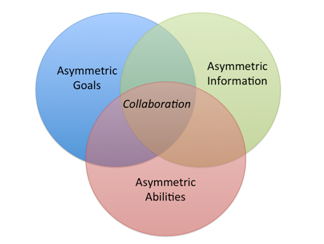
\includegraphics[width=0.4\linewidth]{./fig/collaboration.png}
\caption{Operational Elements of Collaboration.}
\label{fig:collaboration}
\end{figure}

In this team-centered approach, both humans and robots can take on roles that match their strengths. Properly designed, this can facilitate the performance of the entire team.
This idea has already been applied to reform human-robot interaction in many areas, like object identification, collaborative tasks performance, etc. ~\cite{Hoffman2004}. 
We adopt the notion of collaboration, operationally defined as the process of utilizing shared resources (communication, space, time) in the presence of asymmetric goals, asymmetric information, and asymmetric abilities as illustrated in Figure \ref{fig:collaboration}. 
The word collaboration suggests that there are both overlaps and differences between the goals, information, and abilities of the agents involved. Colloquially, collaboration can happen when everyone has something unique to offer and something unique to gain, but there is some benefit to each individual if activity is correlated.

%In a human-robot team, the asymmetries on abilities and information mostly come from the natural difference on agents’ sensors and actuators. 
%Additionally, an agent may exhibit ability and information asymmetry in different states of interacting with the environment, like location, lighting condition etc. 
%Often, a team goal will be decomposed into subgoals in execution. 
%The subgoals are usually assigned to agents in the team by organizing agents into specific roles with specific responsibilities, and this leads to goal asymmetries.

%%%%%%%%%%%%%%%%%%%%%%%%%%%%%%%%%%%%%%%%%%%%%%%%%%%%%%%%%%%%%%%%%%%%%%%%%%%%%%%
%\subsection{Research-Related Work}
\subsection{Algorithm-Specific Work}
% Related Work
% 1-2 pages
% Answers:
% 3) What have others done to solve this problem and why is this inadequate?
%    (only a small overlap with the area exam from the introduction)

In a collaboration framework, the interaction between agents not only focuses on common goals, but may also on supporting others’ goals. 
In a team search tasks, for example, the robot and the human might work together to search for a target, while the robot might assist the human to deal with an emergency.
We will review several problems that are relevant with the information flow to the robot in the human-robot collaboration.
How the robot understands the goal received from the human includes the submodularity, homotopy, multiple objectives and semantics in path planning.

\subsubsection{Path Planning by Human Instruction}

Current human-robot communication relies heavily on the training of the human, which means that the human should program the information for the robot.
This prevents the human-robot interaction applied into more fields.
The goal of current research studies is supporting the robot to understand the natural information from the human.

A typical feature of the human's task description is qualitative, planning algorithms have been thus proposed to generate solutions based on qualitative description~\cite{mcclelland2012qualitative,6425551,mcclelland2014qualitative,shah2013qualitative}.
Uncertainty is involved in modeling the initial map priori.
With more observations in moving, the planned solution can be updated in an online manner.
A more natural and easy way of expression is natural language.
Planners have been proposed to infer the human's intent from the human's verbal instructions~\cite{howard2014natural,Duvallet2014}.
In these planners, groundings are extracted from the semantics in the working environment.
The verbal command is parsed into phrases by Spatial Descriptive Clause. 
The factor graph is then created to model the correspondence between the groundings and the phrases.
Labeled training dataset can be used to train the factor graph model.
After training, the factor graph model can be used to infer the groundings from verbal instructions, which provides the human's intent behind.

\subsubsection{Multiple Objectives in Path Planning}

Many tasks assigned to robots are complex, can be performed in several different ways, and must maximize several different performance objectives.
For example, a robot in a search task may be expected to maximize the area that it covers while minimizing energy consumption and avoiding risk, for example~\cite{Mei2005,Yi2014}. 
As another example, a robot manipulator may need to satisfy performance criteria related to movement, joint velocities, joint accelerations, etc.~\cite{Pires2004}.

A common method for finding a solution to a multi-objective optimization problem is to optimize a single objective created by a weighted sum of the multiple objectives.  
In path-planning the properties of the path produced by this method depend strongly on how each objective is weighted. 
This means that a programmer, designer, or human teammate 
must decide how to assign the weights so that the qualitative behavior matches what is intended.  
In addition to the burden this places on the human operator, optimizing a weighted sum does not work when the multiple objectives are very difficult to compare or are expressed in incommensurate units.

Most popular methods in multi-objective optimization are not naturally applicable to path-planning problems~\cite{Zhang2007,Deb2014}.
One approach to addressing this issue is to change the representation for a path by coding a path as a sequence of fixed-length line segments represented by direction~\cite{Ahmed2013,Howlett2006} or waypoints~\cite{Sujit2009,Pires2004} so that an evolutionary algorithm can be applied. 
Unfortunately, these approaches do not scale well for large problems, and estimating the required number of segments a priori is very challenging. 
Another approach is to represent the path as a point in a very high-dimensional vector space.
In this approach a path is represented as a point in a $ n * d $ dimensional space formed by n d-dimensional way-points.
However the search can be more difficult if we allow the number of way-points, and therefor the dimensionality of the optimization problem, to vary. 
The algorithm we present works when the obstacles in the path-planning space introduce discontinuities in these high-dimensional spaces, which limits the applicability of heuristic-based search approaches~\cite{Sujit2009,Zhang2007}.
There is still the need of an algorithm that can efficiently and effectively find a set of Pareto optimal paths for given multiple objectives.

\subsubsection{Homotopy in Path Planning}

Different from the common optimization problem, the solution of the path planning cannot only be evaluated by fitness but also carries a shape property.
Humans often represent the world using a topological rather than metric-based path planning~\cite{Aginsky1997,kuipers1999}. 
Various methods have been used to create topological-representations that can be used by path-planners for robots~\cite{Mataric1992,Thrun1998,Fasola2013,Shah2013}.
The obstacles in the map divide the paths into topological groups by similarity. 
The topological notion of homotopy presents a formal definition of the similarity between two paths. 
This definition can be used both to determine the similarity between two paths as well as to partition paths into different classes.

Homotopy-based path planning requires an algorithm to determine the homotopic equivalence of two paths, which is usually computationally expensive. 
There are a few research studies that focus on effectively and efficiently identifying the homotopy class to which a path belongs or determining the homotopic equivalence of two paths. 
The Voronoi diagram is used to identify a path from any homotopy class in~\cite{Banerjee2013}. 
By converting any path into a simple path from the Voronoi diagram, the homotopy class of the path can be determined. 
However there exist limitations on finding some paths in a map with complex obstacles in this approach.
By applying the funnel algorithm in the universal covering space, the minimum-length path is efficiently optimized in a given homotopy class in~\cite{Hershberger1994}. 
Similar with the Voronoi approach, the complexity of the problem is increased when the shapes of the obstacles are not smooth and convex. 
Semi-algebraic cuts are used to convert the path into “word” so that the homotopic equivalence can be compared~\cite{Grigoriev1998}. 
The Cauchy Integral theorem has been introduced to determine the homotopic equivalence of any two paths by marking the positions in the obstacles as undefined~\cite{Bhattachary2010}. 
Given two paths sharing the same start and goal, we can determine whether there is an obstacle inside a region that is closed by two paths by the value of the complex integral. 
Because the map is discretized, the computation cost expands greatly if the obstacles are reasonably approximated by the cells.
How to efficiently and effectively find the optimal paths in different homotopy classes is still an open question.

\subsubsection{Submodularity in Path Planing}

In planning motion for a robot in a human-robot team, search is one of the most important tasks that we are interested with.
In planning motion for a search task, the objective is usually to maximize the information collected with a limited motion resource.
Because an observation at a time covers a region near around the search agent, using a coverage model for the robot makes the path planning a {\em maximum coverage problem}.
Maximum coverage is known to be a classic NP-hard combinatorial optimization problem~\cite{Megiddo1983} because coverage overlap can not be ignored. 
Mutual information is introduced to measure the total information
of a set of observation coverages, which implies a property of
“nondecreasing submodularity”~\cite{Singh2009}. 
A greedy approximation with known performance bound can efficiently exploits the submodularity property of mutual information~\cite{Singh2009}. 
A branch and bound approach can also be used in informative path
planning~\cite{Binney2012}.

Maximizing the reward collected from a limited-length graph walk is usually known as an orienteering problem~\cite{Vansteenwegen2011}, in which the total reward is a summation of the rewards of visited vertices. 
If the reward function of a vertex has submodularity as in a maximum coverage problem, the problem is defined as a submodular orienteering problem~\cite{Chekuri2005}. 
Unfortunately in the submodular orienteering case the location of the robot at time t constrains the reachable locations at time t+1.
Thus, naively applying a greedy algorithm to the submodular orienteering case, that is, with a “teleport” assumption, yields poor results~\cite{Krause2012}. 
For a generalization of the submodular orienteering problem in which the neighboring constraint can be converted into time budget, a recursive greedy algorithm can be applied~\cite{Chekuri2005}.
However, when we import the constraints from a human teammate's behavior to the submodular path planning, this solution won't work any more. 


%%%%%%%%%%%%%%%%%%%%%%%%%%%%%%%%%%%%%%%%%%%%%%%%%%%%%%%%%%%%%%%%%%%%%%%%%%%%%%%
\section{Thesis Statement}
% 1 to 2 sentences

Information flow from the human to the robot in a human-robot team is a bottleneck of the team performance.
In a path-planning problem, we are interested with how the robot can understand the human language instructions, how to identify the human's intent among multiple objectives and how to identify the human's topological preference.
We will propose algorithms to solve these problems and show the effectiveness and efficiency of these algorithms.

%%%%%%%%%%%%%%%%%%%%%%%%%%%%%%%%%%%%%%%%%%%%%%%%%%%%%%%%%%%%%%%%%%%%%%%%%%%%%%%
\section{Project Description}
% about 6-8 pages
% Answers:
% 4) What is your proposed solution to this problem?

We will model the following aspects of information flow from the human to the robot, which includes 
\begin{itemize}
\item how to identify the human's intent when finding trade-offs among multiple objectives,
\item how to recognize the human's topological preference, and
\item how to model the problems from humans' language instructions,
\end{itemize}
After they have been modeled into path planning problems, we will propose algorithms to solve the problems and provide analyses and simulations to support the algorithms.

\begin{table}[h]
\begin{center}
{\renewcommand{\arraystretch}{3}
\begin{tabular}{|l|l|l|l|}
	\hline
	\multicolumn{2}{|l|}{ \textbf{Requirement} } & \textbf{Problem} & \textbf{Algorithm} \\ \hline
	\multicolumn{2}{|l|}{ \pbox{20cm}{Identify the human's intent on\\ multiple objectives} }  & Multi-objective path planning & MORFF $^{*}$ \\ \hline
	\multicolumn{2}{|l|}{\multirow{2}{*}{ \pbox{20cm}{Recognize human's topological\\ preference} }}  & \pbox{20cm}{Submodular path planning with \\ reference path constraint} & Wingman path planning \\ \cline{3-4} 
	\multicolumn{2}{|l|}{ }  & Homotopy-based path planning  & HA-RRT$^{*}$ \\ \hline
	\multicolumn{2}{|l|}{ \pbox{20cm}{Model problems from verbal\\ instructions} } & \pbox{20cm}{Grounding multiple objectives and \\ topological preference in \\ natural language} & \pbox{20cm}{ DCG (Distributed \\ Correspondence Graph)} \\ \hline
\end{tabular}
}
\end{center}
\label{tb:requirement}
\caption{Project description.}
\end{table}

\subsection{Multi-Objective Path Planning}

To support the complex decision with multiple objectives, we define the multi-objective path planning and propose the algorithm to find the solutions.

When there are multiple objectives in a task, the goal is finding a solution that balances between different objectives.
A common method for finding a solution to a multi-objective optimization problem is to optimize a single objective created by a weighted sum of the multiple objectives.
This means that either the programmer, designer , or a human teammate must decide how to assign the weights so that the qualitative behavior matches what is intended. 
Optimizing a weighted sum does not work when the multiple objectives are very difficult to compare or are expressed in incommensurate units.

Consider a multi-objective path planning problem defined on a bounded, connected open set $X\subset\mathbb{R}^d$ of possible solutions, and $K$ different objectives $\{c_{1}(\cdot), c_{2}(\cdot), ... c_{K}(\cdot)\}$. 
Without loss of generality, assume that each $c_{k}(\cdot)$ is a cost function such that the objective is to minimize these functions.  
Since the Pareto optimal set is not enumerable, the {\em goal is to find a representative, finite ($M$-element) subset of the Pareto optimal set}.  
By ``representative" we mean a diverse set of solutions that span the Pareto set rather than, for example, several points clustered in a single region of the Pareto set.

In contrast to searching through and comparing solutions in order to find the Pareto optimal set, we use a decomposition-based method similar to MOEA-D~\cite{Zhang2007}.  
MOEA-D is an algorithm that decomposes a multi-objective optimization problem into a set of subproblems.  
Each subproblem uses a weighed combination of the objectives to find specific points in the Pareto set or to guide the search for such points.  
%Because we  will use this subproblem idea in our algorithm, it is useful to introduce some notation.
Let $ \bm{\lambda} = [ \lambda_{1} , \cdots , \lambda_{K}  ]^{T} $ be a weighting vector such that $ \sum_{k=1}^{K} \lambda_{k} = 1 $.  
Let $\{c_{1}(\cdot), c_{2}(\cdot), \ldots c_{K}(\cdot)\}$ denote the $K$-element set of objective functions, let $\bm{c}(x) = [c_{1}(x), c_{2}(x), \ldots, c_{K}(x)]^T$, and let $x$ denote a potential solution.  
Finally, let $ \bm{z}^{\rm utop} = [z^{*}_{1}, \cdots , z^{*}_{K}]^{T} $ denote the so-called Utopia reference vector. %, described in more detail in the next section. 
Three types of decomposition methods have been used in prior work~\cite{Zhang2007}.
\begin{eqnarray}
\arg\max_x \sum_{k=1}^{K} \lambda_{k} c_{k} (x) & {\rm weighted \ sum} \label{eq:weighted}\\
\arg\min_x\max_{1 \leq k \leq K}  \{ \lambda_{k} \mid c_{k}(x) - \bm{z}^{\rm utop}_{k}  | \} & {\rm Tchebycheff} \label{eq:Tchebycheff}\\
\arg\min_x \{ d \mid \bm{z}^{\rm utop} - F(x) = d \bm{\lambda} \} & {\rm boundary \ intersect\ } \label{eq:boundary}
\end{eqnarray}
The solutions generated by each method are a subset of the Pareto optimal set.

\begin{figure}[htbp]
	\centering
	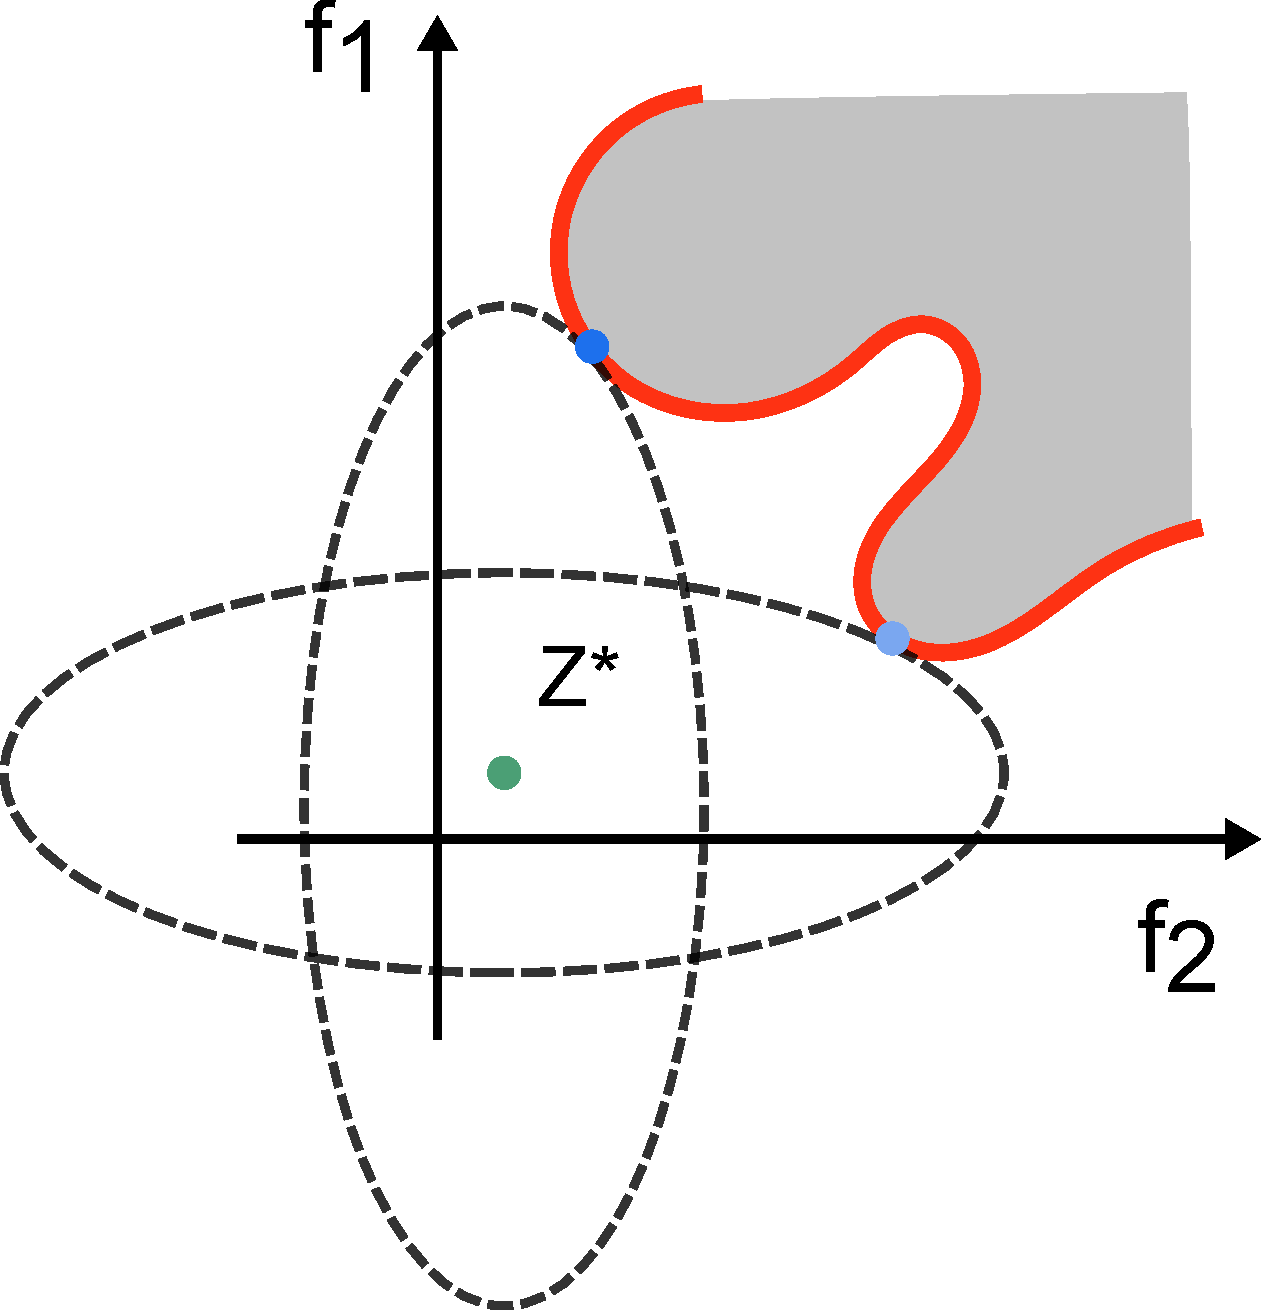
\includegraphics[width=0.3\linewidth]{fig/Tchebycheff}
	\caption{Tchebycheff method of finding Pareto front.}
	\label{fig:Tchebycheff}
\end{figure}

We propose an algorithm that explores the solution space using RRT$^{*}$-based tree structures but uses multiple trees in the spirit of decomposition-based multi-objective optimization.
Because a set of trees are constructed in the exploration process, we call the algorithm MORRF$^{*}$ (Multi-Objective Rapidly exploring Random Forest$^{*}$).

\begin{figure}[htbp]
	\centering
	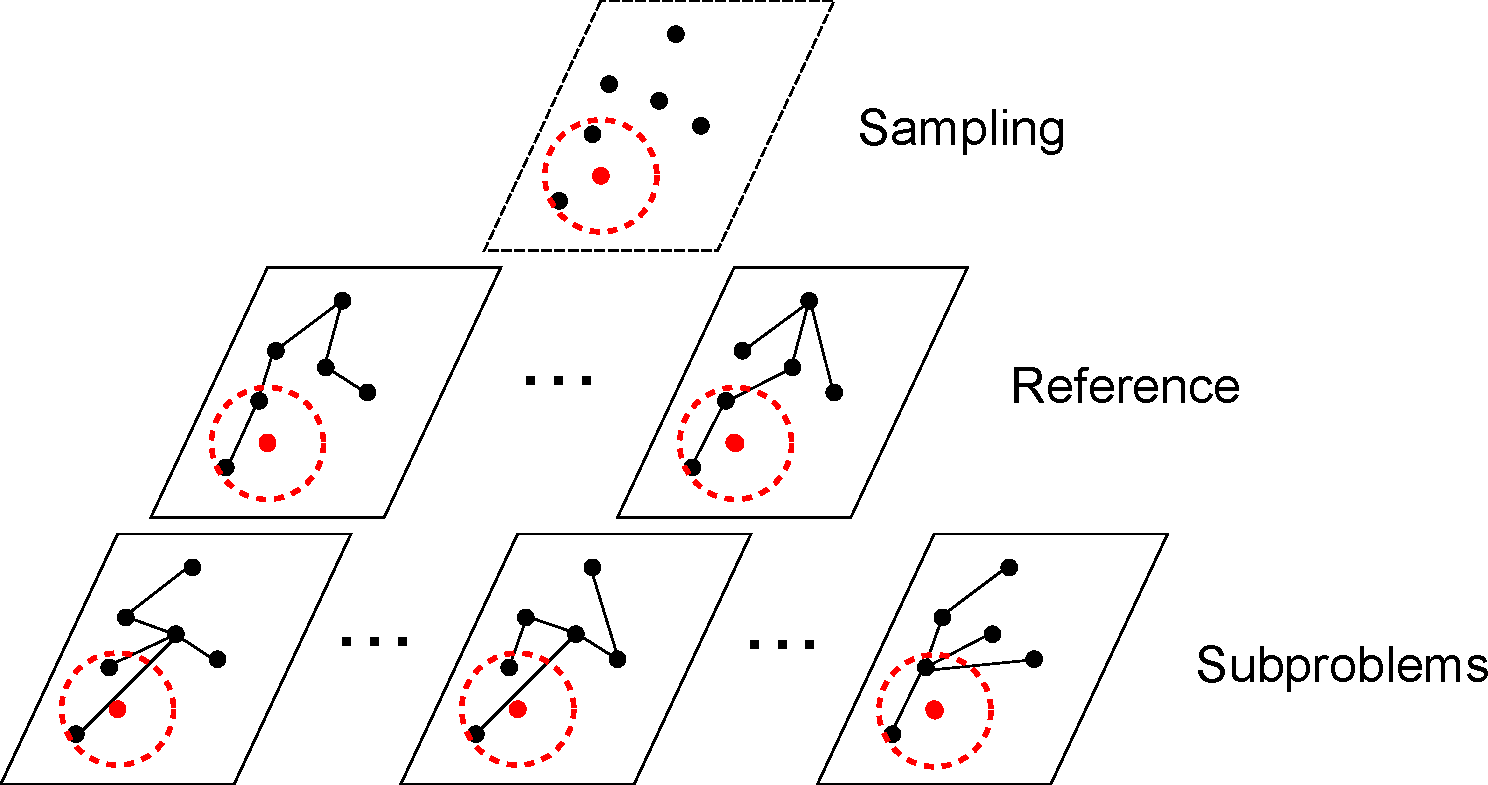
\includegraphics[width=0.55\linewidth]{./fig/MORRTstar}
	\caption{Rapidly exploring process}
	\label{fig:MORRTstar}
\end{figure}

Adopting the idea from the MOEA-D algorithm~\cite{Zhang2007}, the $M$ elements in the solution set $\Sigma^{*}$ will be obtained by decomposing the multi-objective problem into $ M $ subproblems.  
Both the Tchebycheff approach and Boundary Intersection approach require us to define a Utopia reference vector $ \bm{z}^{\rm utop} $ in the fitness space. 
Figure~\ref{fig:Tchebycheff} illustrates how this reference vector is used in a simple (not path planning) two objective problem.  

Take the Tchebycheff approach as an example.
Recall that  $ \bm{\lambda} = [ \lambda_{1} , \cdots , \lambda_{K}  ]^{T} $ is a weighting vector such that $ \sum_{k=1}^{K} \lambda_{k} = 1 $ and that the Tchebycheff approach seeks to find the solution $ x^{te}\in X $ given by $ x^{te} = \arg\min_x \max_{1 \leq k \leq K}  \{ \lambda_{k} | c_{k}(x) - \bm{z}^{\rm utop}_{k}  | \} $.  
As illustrated in Figure~\ref{fig:Tchebycheff}, the Utopia reference vector is defined as the point in cost space that would be obtained if it were possible to find a solution that produced the minimum value for all objectives, that is the $k^{\rm th}$ element of $\bm{z}^{\rm utop}$ is given by $\bm{z}^{\rm utop}_{k} = \arg \min_{x \in X} c_{k}(x)$.  
It is called the ``Utopia'' reference vector because it represents a point that very best that could conceivably be achieved for an ideal point in the solution space.

Given this brief overview of the Tchebycheff method, we now need to extend it to allow for RRT$^{*}$-based sampling of the search space.  
We will need one type of RRT$^{*}$ structure to explore in an attempt to find the Utopia reference vector in payoff space and another type of RRT$^{*}$ structure to find paths that minimize the Tchebycheff condition. %, as described below.  
Thus, there are two types of tree structures used for the optimization process.
\begin{itemize}
	\item Each \emph{reference tree} explores using a single objective $ c_{k} (x), k \in K $. 
	The cost of each vertex is calculated using the $ k^{\rm th} $ objective function.
	\item Each \emph{subproblem tree} explores a subproblem $ g_{m} ( x \mid \lambda_{m} , \bm{z}^{\rm utop} ) , m \in M $.
	The cost associated with each vertex is calculated using $ g_{m}(x) $ defined by the corresponding approach.
\end{itemize}
Thus $ K $ reference trees are used, one each to explore the minimum of each objective, and $ M $ subproblem trees are used, one for each weighting vector, $ \lambda_{m} $.  
The $K$ reference trees and $M$ subproblem trees constitute the exploration forest.
The solutions obtained from $ M $ subproblem trees constitute a set of Pareto optimal paths, which is the solutions to the multi-objective path planning problem. 


\subsection{Involving Topological Preferences in Path Planning}

We categorize the topological preference into two types by considering the level of collaboration.
If the human and the robot are constrained in a tight collaborative relationship, the motion of the robot has to be constrained in a region near around the location of the human.
The topological preference is defined by a reference path from the human.
By considering the sensor coverage overlap in collaboration, we can model the problem into submodular path planning with reference path constraint in Section~\ref{sec:submodular_path_planning_with_reference_path_constraint}.
If we ignore the collaboration, the topological preference can then be presented by the homotopy classes in the map.
Therefore, in this case, we can model the problem into homotopy-based path planning in Section~\ref{sec:homotopy_based_path_planning} 

 

\subsubsection{Submodular Path Planning with Reference Path Constraint}
\label{sec:submodular_path_planning_with_reference_path_constraint}

Before the task execution, the coach assign a subtask to a robot player as the goal.
The information of another human player might also be given for the planning purpose.
If the human player's motion can be predicted or known and the robot player's motion is constrained by the human player's motion, we have a path planning problem with reference-path constraint.
We consider this situation in a search task with the robot wingman.

Consider a discretized map of the world formed by a set of cells $ \mathbf{S}$ and suppose that the robot moves with constant speed from a cell to its neighbors.
In the search task, each cell in a discretized map is assigned an entropy value to represent the information distribution.
The robot's motion is constrained by a graph topology determined by the cell neighborhood. 
In a period of time of length $ T $, we denote the robot's path as $ X = [x_{1}, x_{2} , \cdots , x_{T}] $.
We adopt an observation coverage model for the robot, which means that the robot can observe not only the cell it currently occupies but also neighboring cells within a given range.
Let the observation at time step $ t $ be $ O^{X}_{t} $, which describes both the observed cells and how well they are observed.
Thus the robot's path, $X$, induces a sequence of observations $ \mathbf{O}^{X} = \{ O^{X}_{1}, \cdots , O^{X}_{T-1}, O^{X}_{T} \}$.

We assume that the observation coverage model follows Bayes rule.
Thus we can define the information gain of the robot using mutual information $ I( \mathbf{S} \mid \mathbf{O}^{X} ) =  H( \mathbf{S} ) - H( \mathbf{S}, \mathbf{O}^{X}  ) $.
The entropy reduction over the problem space $ \mathbf{S} $ by the observation $ \mathbf{O}^{X} $ is the {\em information gain} to the robot.

\begin{figure}[hbtp]
\centering
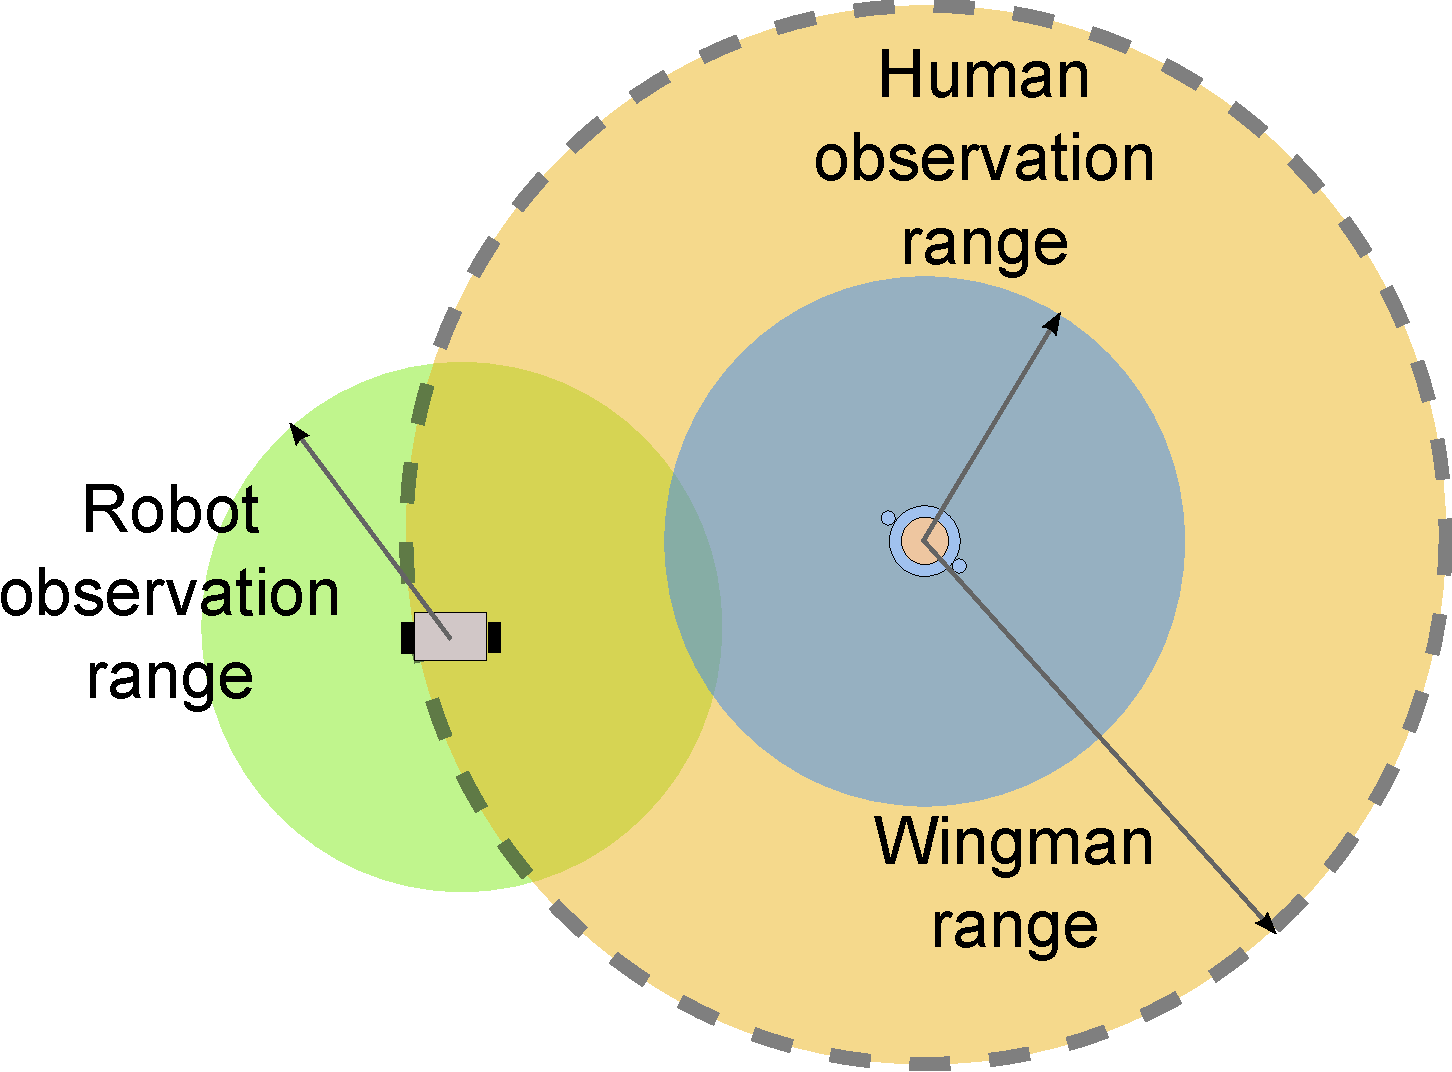
\includegraphics[width=0.37\linewidth]{./fig/Wingman.pdf}
\caption{A Robot Wingman Framework.}
\label{fig:Wingman}
\end{figure}

We select the wingman as a role for the robot player, though there are a few ways that a human can constrain the robot's path.
The wingman role requires that the robot player stands in a range near around the human player while the human player is moving, as in Figure \ref{fig:Wingman}.
Assume we have a model that can predict the human's path.
We denote the human's $T$-step path as $ Y^{h} = [y^{h}_{1}, y^{h}_{2} , \cdots , y^{h}_{T}] $.
We define a neighbor function $ N () $ that represents the assumption from the introduction that the robot can deviate from a constrained path by no more than a given tolerance.  
At each time step, this neighborhood induces the set of {\em visitable cells} for the robot, which is denoted by $ N( y^{h}_{t} ) $.
Figure \ref{fig:humanConstraint} gives an example.
By organizing the set of visitable cells at time $ t $ into a partition of vertices, we can construct a multi-partite graph $ G = (V, E, T) $ from the constrained path.
A partition $ V(t) \in V $ is obtained from the cells in $ N( y^{h}_{t} ) $.
The edge set $ E $ is determined by the neighborhood of each cell from the discretized map.

Imposing the path constraint $ Y^{h} $, we define the multi-partite graph as follows.
Figure \ref{fig:MultiPartite} illustrates how the path constraint induces the multi-partite graph for a notional human path.
Note that a cell in the discretized map might appear in multiple partitions due to overlaps between sets by $ N( y^{h}_{t} ) $ at different $ t $.

\begin{figure}[htbp]
	\centering
	\begin{subfigure}[t]{0.45\linewidth}
		\centering
		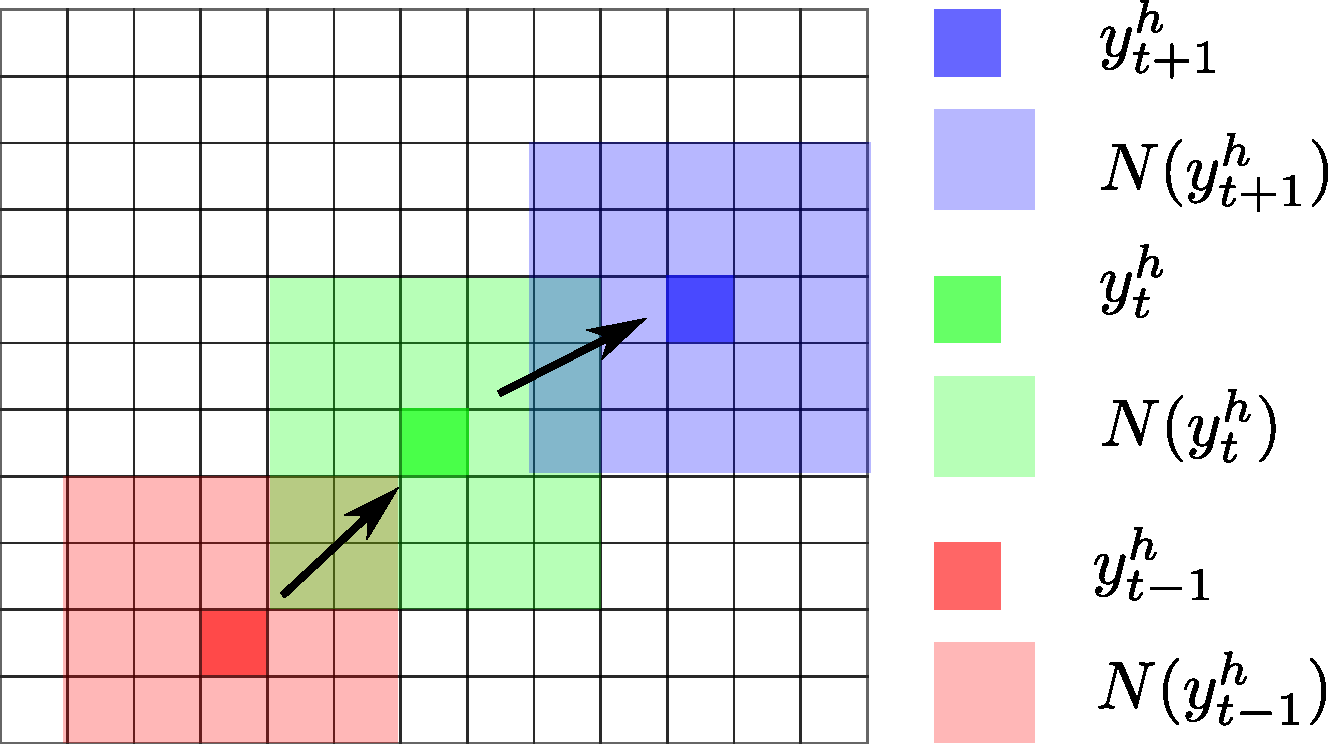
\includegraphics[width=\textwidth]{fig/humanConstraint.pdf}
		\caption{How the multi-partite graph is obtained..}
		\label{fig:humanConstraint}
	\end{subfigure}  
	%\\
	\begin{subfigure}[t]{0.45\linewidth}
		\centering
		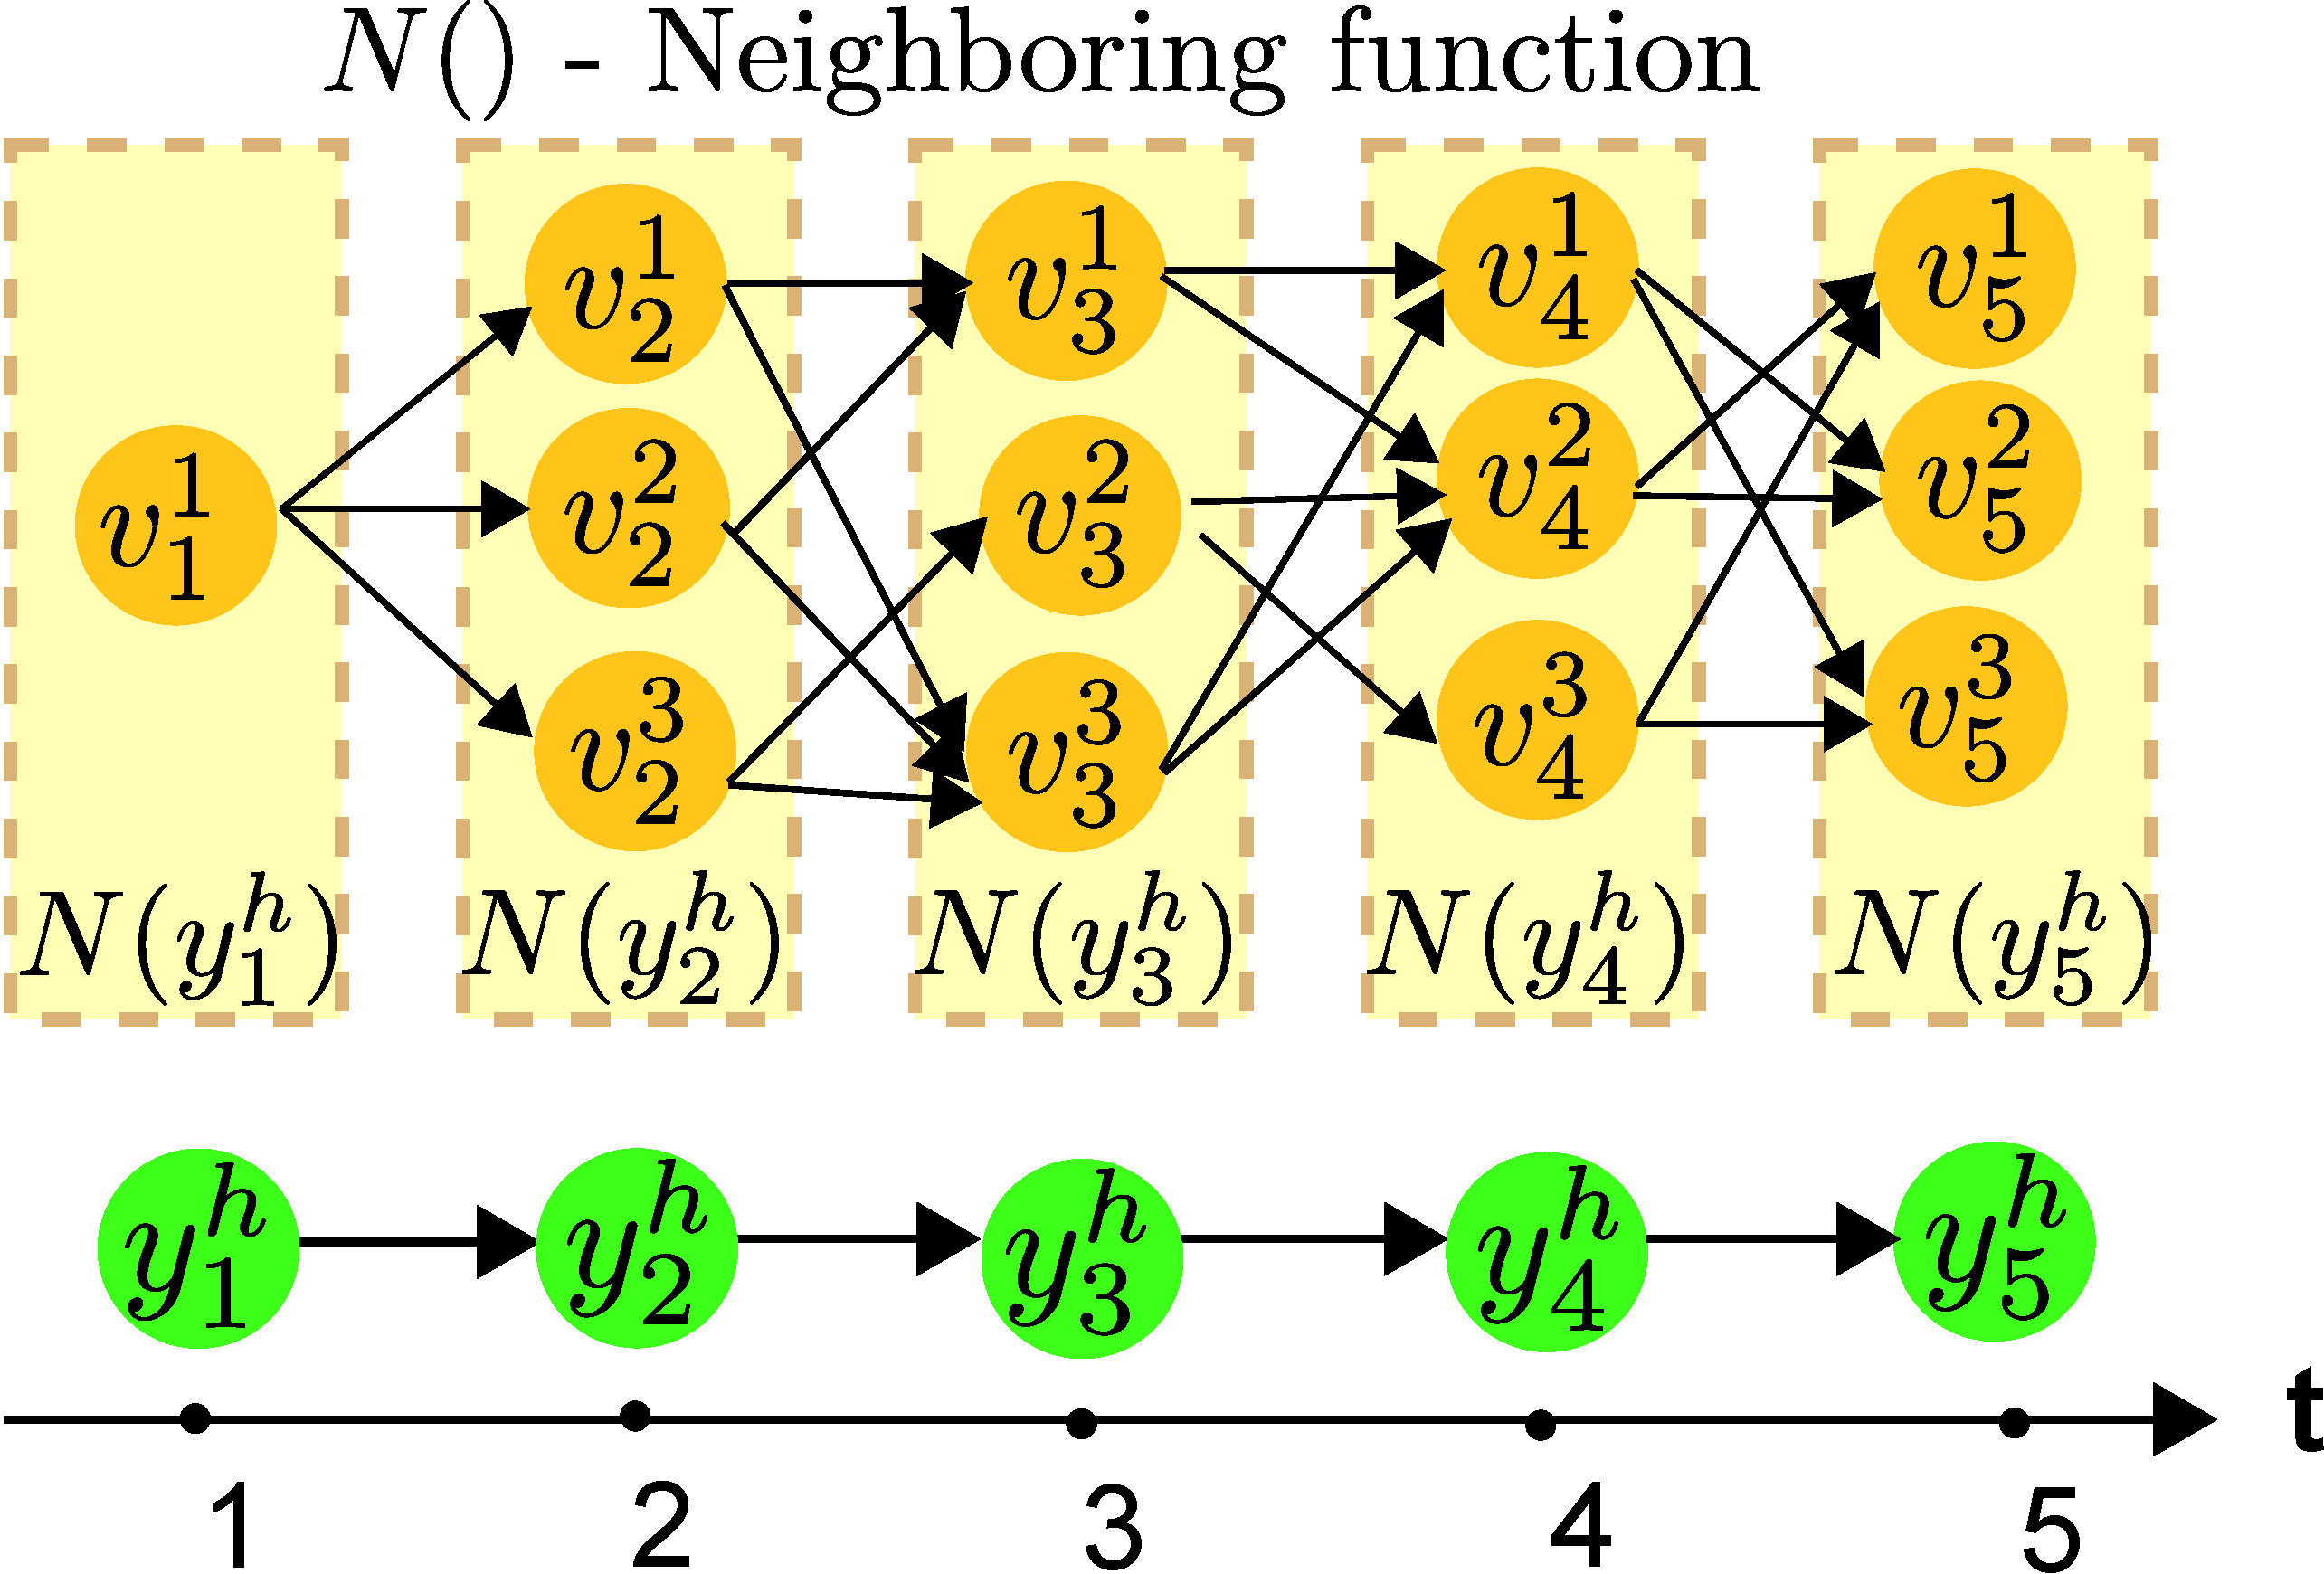
\includegraphics[width=\textwidth]{fig/MultiPartite.pdf}
		\caption{A multi-partite graph from a human path constraint.}
		\label{fig:MultiPartite}
	\end{subfigure}   
	\caption{Reference constraint.}
	\label{fig:reference_constraint}
\end{figure}

In order to guarantee that the search process on a multi-partite graph $ G = (V, E, T) $ always ends with a path of length $ T $, we use a pruning process to ensure that each vertex can be reached from the previous partition and is connected to a vertex in the next partition.
we use backtracking to estimate the maximum total reward and use this estimate as our search heuristic.
We then use an expanding tree to create an anytime algorithm approximate solution to the submodular orienteering problem on the multi-partite graph.

\subsubsection{Homotopy-based Optimal Path Planning}
\label{sec:homotopy_based_path_planning}

We also notice that, in planning the path for the robot player, some of the preferences on the paths for the subtask might be hard for the coach to express.
Topology of a path is one of the factors that are hard to model into the quantitative models.
The topological concept of \emph{homotopy} is a mathematical formalism of the inherent similarity or dissimilarity of two paths.
Given two paths, if one can be deformed into the other without encroaching any obstacle, they are said to be \emph{homotopic}~\cite{Hernandez2015}.
The set of paths that are homotopic to each other form a \emph{homotopy class}, and the  set of homotopy classes partition the set of all possible paths between any two points $A$ and $B$.
In an environment containing obstacles, the homotopy partition can provide a useful way of grouping paths together based on the similarities of their ``shapes," where the term ``shape'' is interpreted using the formal topological notion.

In order to support these forms of human intents, expressed as homotopic constraints and preferences, we propose a homotopy-aware RRT$^{*}$ (HA-RRT$^{*}$) algorithm. 
This algorithm uses an RRT$^*$ algorithm to explore possible paths, but each branch of the random tree is aware of the homotopy class to which it belongs. 
We use a set of reference frames for homotopy class identification.
Figure \ref{fig:obs_map:map} shows an example of a map that is decomposed with the reference frames (blue and green dash lines).
A \emph{reference frame} is defined as a line segment that connects either two obstacles or an obstacle and a boundary.
A topological graph can be created by the connectivity of the decomposed regions.
Each region from the map decomposition is a node in the topological graph.
Each reference frame is adjacent to two regions; thus, it becomes an edge that connects two nodes.
Figure \ref{fig:obs_map:topology} shows a topological graph from the map decomposition in Figure \ref{fig:obs_map:map}.

\begin{figure}[htbp]
	\centering
	\begin{subfigure}[t]{0.27\linewidth}
		\centering
		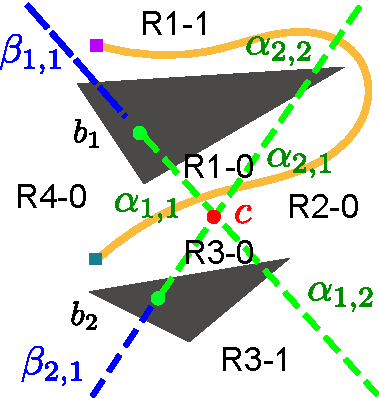
\includegraphics[width=\textwidth]{fig/obs_map.pdf}
		\caption{Decomposition of the map with obstacles.}
		\label{fig:obs_map:map}
	\end{subfigure}  
	%\\
	\begin{subfigure}[t]{0.27\linewidth}
		\centering
		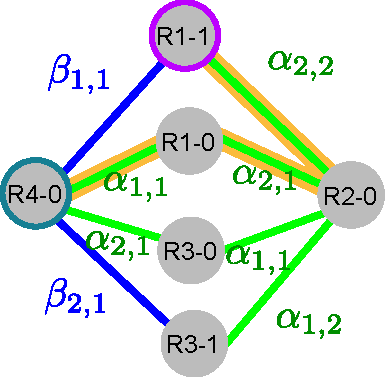
\includegraphics[width=\textwidth]{fig/obs_topology.pdf}
		\caption{The generated topological graph.}
		\label{fig:obs_map:topology}
	\end{subfigure}   
	\caption{Map with obstacles.}
	\label{fig:obs_map}
\end{figure}

Label each reference frame with a \emph{character}.
Each path can be mapped into a {\em string}, which represents the sequence of the crossed reference frames.
In \cite{Hernandez2015}, the string is used to identify the homotopy class of each branch in the RRT so that the growth of a tree is constrained in a homotopy class, because starting from the root of the tree to each branch makes a subpath.
We have each branch of the tree structure tracking the corresponding string as the homotopy information, so that the homotopic constraints can be satisfied or the homotopy class can be identified.

We define the paths with same string as a \emph{string class} and use $ - $ to concatenate characters into a string.
Two string classes might still belong to the same homotopy class, e.g. a string class $ \alpha_{1,1}-\alpha_{2,1} $ and a string class $ \alpha_{2,1}-\alpha_{1,1} $ by the reference frames in Figure \ref{fig:obs_map}.
A homotopic grammar is needed to identify the equivalence.
Also, the homotopic grammar can be used to find all the equivalent string classes in the same homotopy class by giving one string class.

With the generated reference frames $ \mathbf{R} $ to identify the homotopy classes, the next question is how to search the optimal paths in the homotopy classes.
RRT$^{*}$ explores the map to generate an optimal tree structure based on the cost distribution in the map.
The homotopy-based path planning problem essentially looks for the optimal solutions with the constraints of visiting different regions.
Because a single optimal tree structure only explores one and only one global best, it cannot support the finding of the optimal solutions of multiple classes.
We use a bidirectional RRT$^{*}$ to obtain the optimal cost-to-come and cost-to-go for different positions.
We can eventually have the optimal path with a via-position constraint by combining the optimal cost-to-come to the via position and the optimal cost-to-go to the via position.
Because the string classes of the branches of both two trees are also tracked in the exploration process, the optimal path that visits a specific via position can be used to update the optimal paths of the string classes. 
Thus, in the exploration process, the homotopy classes of each branch of the tree are aware.

\subsection{Path-Planning with Natural Language Instruction}

An important way for a human to command a robot is through natural language.
We need to provide methods to infer the task definition from the human's language, focusing on the requirements on multiple objectives and topological preferences.
As we are interested with robotic path planning, we will focus on how to model the optimization problems from the human's verbal commands.
We will emphasize on the multiple objectives and the topological preference.
For example, if the human coach tells the robot that ``go around building A quickly and carefully and then between the two trees while avoiding region C'',
it implies that there potentially exist two objectives from the adverb, ``quickly'' and ``carefully''.
In a military application, it might mean to minimize the path length and minimize the risk.
It also indicates the topology of the path that the human wants, which needs ``around building A'', ``between the two trees'' and ``avoiding region C''.

The graphical model has been a popular tool to model the ambiguous relationship between the natural language and the semantics.
After training from the language samples, the graphical model could infer the meaning of verbal language.
Similarly, we can use this to understand the human's verbal commands to the robot.
In path planning problem, the human's verbal commands deal with the spatial elements. 
Spatial descriptive clause(SDC) is introduced to parse the verbal command into a sequence of phrases~\cite{Kollar:2010:TUN:1734454.1734553}.

The process of assigning physical meanings to natural language is called {\em grounding}.
A verbal sentence is decomposed into phrases $ \lambda^{r}_{i} $, which carry the information from the human.
Grounding variables $ \gamma^{r}_{j} $ are extracted from the map, which include
\begin{itemize}
\item {\em verb fields} : the change in orientation between viewpoints from verb/action semantic;
\item {\em figure and landmark fields} : the viewpoint transition and detected objects ;
\item {\em spatial relations} : the functions of the geometry of the path and landmark.
\end{itemize}
By assuming that the groundings are conditionally independent, conditional random field(CRF) is used as undirected graphic model to model the relationship between the phrases and the groundings.
Correspondences $ \phi^{k} $ are introduced to indicate whether a grounding element is linked with a phrase from SDC~\cite{tellex2011understanding},
indirectly, it measures how the grounding variables match the verbal sentence.
Figure \ref{fig:graph_model:induction} gives two examples of how graphical models are created from the SDCs.
Corresponding nodes $ \phi^{k} $ connects the grounding nodes $ \gamma^{r}_{j} $ and the phrase nodes $ \lambda^{r}_{i} $.
Labeled dataset can be used to train the graphical model.
The objective of the training is to maximize the likelihood of the correspondences.
\begin{equation}
\arg \max_{\phi_{i,j} \in \Phi } \prod p( \phi_{i,j} \mid \gamma^{r}_{j} , \lambda^{r}_{i} )
\end{equation}
The trained graphical model can then be used to infer the most likely grounding nodes from a given verbal command.

\begin{figure}[htbp]
	\centering
	\begin{subfigure}[t]{0.45\linewidth}
		\centering
		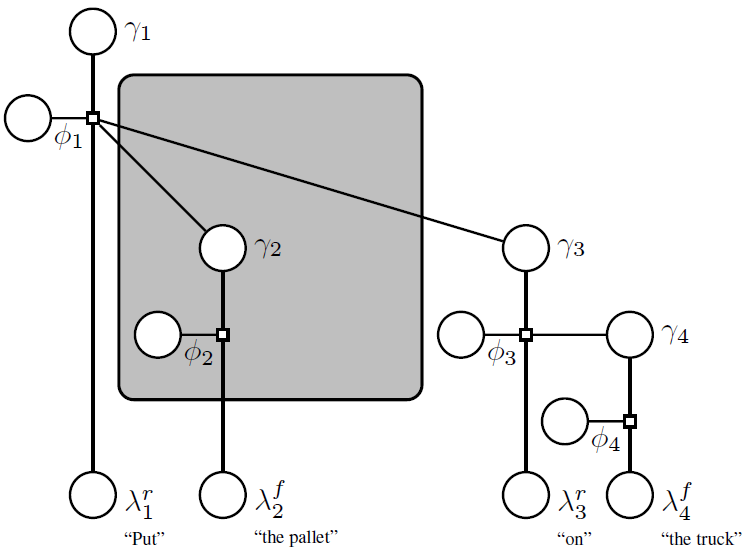
\includegraphics[width=\textwidth]{fig/Induction1}
		\caption{``Put the pallet on the truck.''}
		\label{fig:graph_model:induction1}
	\end{subfigure}  
	%\\
	\begin{subfigure}[t]{0.45\linewidth}
		\centering
		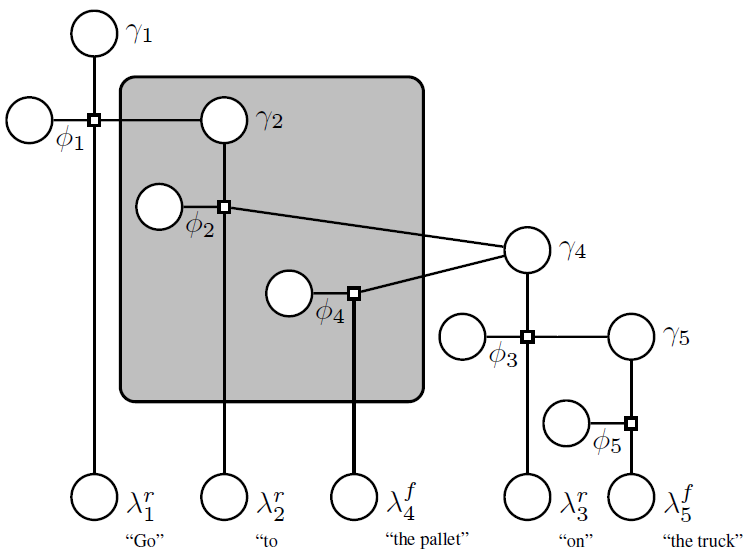
\includegraphics[width=\textwidth]{fig/Induction2}
		\caption{``Go to the pallet on the truck.''}
		\label{fig:graph_model:induction2}
	\end{subfigure}   
	\caption{Graph model of two examples.}
	\label{fig:graph_model:induction}
\end{figure}

It is noticeable that some adverb might mean differently with different verb in different scenario.
For example, in a sentence of ``put the pallet carefully on the truck'', ``carefully'' indicates a smooth motion. 
But in a sentence of ``walk carefully in the crowd'', ``carefully'' means avoiding collision to someone else.
The adverb can also lead to multiple objectives as well, e.g. smoothly moving and collision avoiding simultaneously.
The human language understanding process helps identify the human's intent behind.
We can create a factor graph to model the correspondence between the adverbs and the intended objectives in different sentences and scenarios.
After training, it can be used to infer what kind of objectives the human intended in the verbal command.

Similarly, the topological preference can be recognized from the human language.
In~\cite{howard2014natural}, the topological preference is inferred from the human language and is used as the hard constraint in path planning.
Sometimes, the topological preference can be sort of a soft constraint.
For example, if the human coach says ``better avoiding region C'', he means to prefer avoiding region C but not necessarily.
The topological preference can also be the order of different homotopy classes.
``Going through between A and B is better than between A and C'' implies a homotopy class via the region between A and B is better than a class via the region between A and C.
We can construct a factor graph to construct the preference relationship between the groundings and the verbal phrases.
The {\em correspondence} nodes are replaced with the {\em preference} nodes.
The preference variable is a real value instead of a boolean value.


%%%%%%%%%%%%%%%%%%%%%%%%%%%%%%%%%%%%%%%%%%%%%%%%%%%%%%%%%%%%%%%%%%%%%%%%%%%%%%%
\section{Validation}
% 1-2 pages
% Answers:
% 5) How can you demonstrate that this is a good solution?

We will formally validate each proposed algorithm by theoretical analyses and experiments.
Theoretical analyses and proofs will be used to support the validity and the performance of the algorithms.
Experiments and simulations will be taken to support the performance of the algorithms.

\subsection{Multi-Objective Path Planning}

We prove that the solutions found by the proposed MORRF$^{*}$ can almost surely converge to be Pareto optimal.
The proof is split into several steps.
First, it is proved that the multi-objective path planning problem can be decomposed into a set of weighted subproblems;
the path from each subproblem is a Pareto optimal path.
Second, we prove that the solutions of MORRF$^{*}$ almost surely converge to the answers of the weighted subproblems.
There are two converging processes, the convergence of the reference trees and the convergence of the subproblem trees.
The convergence of the subproblem trees depends on the convergence of the reference trees.

We then present a series of simulation studies that provide evidence that MORRF$^{*}$ produces a representative set of samples from the Pareto set.
Results from MORRF$^{*}$ are obtained for path-planning problems with two objectives and three objectives, and are compared to a modified version of the NSGA-II multi-objective path-planning algorithm~\cite{Ahmed2013} as well as a variant of MORRF$^{*}$ that uses a weighted sum approach.
NSGA-II was selected because evidence suggests that it provides more uniform samples from the Pareto set than other approaches~\cite{Deb2002}.

\subsection{Reference Path Constrained Optimal Path Planning}

We theoretically prove the convergence of the solution to the optimal.
The proof is split in two steps.
The first step is proving that the backtracking process proposed will never underestimate the maximum reward by utilizing the submodular property of the problem.
The next step is showing that given enough run time, the proposed algorithm can always find an optimal solution.
This is proved by showing that a proposed pruning process will never ``froze'' a node that is in the optimal path.
By the proof of contradiction, we can show that the optimal path can always be found if there is enough run time.

We apply the experiment in a world of hexagonal cells, which is discretized from two-dimension search space.
We define several metrics to measure the performance of the proposed algorithm.
We use a \emph{fully expanded tree size} to measure the \emph{problem size}, which depends on the planning length and the vertex connectivities.
Due to the human constraint, the planning length is determined by the human's path length.
The performance of the heuristic is measured by the \emph{percentage of optimal at first iteration}, that is a percentage computed from the value obtain in the first iteration of the proposed algorithm over the optimal value.
We use the \emph{percentage of nodes explored} to indicate the efficiency of the anytime algorithm framework.
In particular, we are interested in whether freezing nodes improves search efficiency.
In the anytime algorithm, the exploration might not stop when the optimal is found, due to the existence of overestimation.
If current best of a search can reach the optimal very quickly, it means that a best solution found in a fixed time has high probability of being optimal.
We use the \emph{number of iterations reaching optimal (normalized)} to measure this optimal search capability of the proposed algorithm.

The backtracking heuristic is compared with the greedy heuristic in experiments to show the advantage of the performance.
We test the algorithms with different types of workspaces and different types of human reference paths to show the robustness of the performance.


\subsection{Homotopy-based Optimal Path Planning}

We will provide theoretical proof that the proposed algorithm could find the optimal solutions of all the given homotopy classes.
We will show that with the support of a bidirectional tree structure, the solutions of HA-RRT$^{*}$ gradually converge to the best paths in the given homotopy classes.
The proof depends both the trees from two directions converge to optimal structures so that we can have the optimal subpaths from a given via-position to the start and the goal respectively.
The concatenation of the two optimal subpaths makes the optimal path from the start to the goal with the given via-position.
As we can identify the string class that each path belongs to, we can have the optimal paths in each string class.
By the homotopic grammar, we can have the optimal path of each given homotopy class.

We also implement experiments to show how the HA-RRT$^{*}$ can support the sliding autonomy in different levels of human intent on the topology.
Consider the following list of ways in which a human can express intent about path shape, and the corresponding homotopy-based constraint:
\begin{enumerate}
\item \emph{I want the path to visit a sequence of specific regions.}
\item \emph{I want the path to visit some regions and avoid other regions.}
\item \emph{I prefer some path shapes over others, but I recognize that trade-offs may be needed.} 
\item \emph{I have preferences over paths, but I need help in understanding these preferences.}
\end{enumerate}

\subsection{Understanding Verbal Command}

%The validation of how the human information can be understood by the robot includes both theoretical analyses and experiments.

%The theoretical analyses will focus on the validity of the algorithm designs and the performance of the algorithm.
%The experiment will be taken on the gazebo simulator or the turtlebot.
%The experiment will be designed to support the theoretical results and to compare the performance in different cases.
How the robot understands the verbal command is essentially a machine learning problem.
There will be training dataset and testing dataset.
We will verify the learning capability of the proposed factor graph structure.
We will propose the measurement method for calibrating how well the human's intent is identified.
Based on the measurement of intent identification, we can collect the successful rate from the statistics.
The performance of the factor graph can be supported by the successful rates of the training dataset and the testing dataset.

\section{Appendix}

We analyze the consensus reaching problem in a team of autonomous agents.
As learned the spirit from \cite{1470210}, we introduce input-to-state stability analysis~\cite{Jiang2001} to each agent in the system, which assists the analysis of the consensus reaching.
We apply it to the Particle Swarm Optimization problem(PSO).
In PSO, each particle is an independent agent.
Each particle has its own subtask, which is seeking the optimal.
For the purpose of the subtask, random factors are imported to the search dynamics.
At the same time, each particle maintains a local information (a personal best) and receives the neighboring information (a global best).
The consensus reaching is that all the particle agree with where the optimal is, so that they share the same global best and personal best.
This is usually called the convergence of the particles.

Although the input-to-state stable analysis can be applied to many versions of PSO,
for this work we use the formulas from Kennedy's most recent definition of PSO~\cite{Bratton2007} for the constricted position-update rule. 
The constricted position-update rule is

\begin{subequations}
\label{eq:pso_alg}
\begin{equation}
\label{eq:up_vel}
\begin{aligned}
v_{ij}(k+1) = \chi [ v_{ij}(k) 
+ \phi^{P} u^{P}_{ij}(k) (x^{P}_{ij}(k) - x_{ij}(k))
 + \phi^{G} u^{G}_{ij}(k) ( x^{G}_{ij}(k) - x_{ij}(k)) ],
\end{aligned}
\end{equation}
\begin{equation}
\label{eq:up_pos}
x_{ij}(k+1) = x_{ij}(k) + v_{ij}(k+1).
\end{equation}
\end{subequations}
$ x_{ij}(k) $ represents the position of particle $ i $ in dimension $ j $ at time $ k $.
Similarly, $ v_{ij}(k) $ represents the velocity of particle $ i $ in dimension $ j $ also at time $ k $.
$ x^{G}_{ij}(k) $ and $ x^{P}_{ij}(k) $ are global best and personal best positions observed by the swarm and the particle respectively. 
$ u^{G}_{ij}(k) $ and $ u^{P}_{ij}(k) $ are independent random values drawn from $ [0,1] $.
$ \chi \in ( 0, 1 ) $, $ \phi^{P} $ and $ \phi^{G} $ are algorithm parameters.

\begin{figure}[htbp]
	\centering
	\begin{subfigure}[t]{0.6\linewidth}
		\centering
		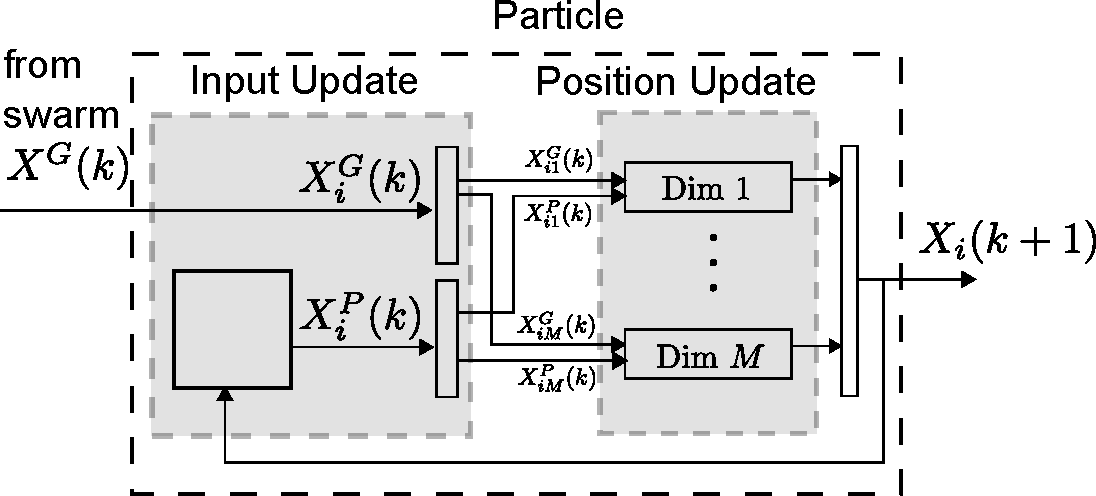
\includegraphics[width=\textwidth]{fig/particle_sys_flow.pdf}
		\caption{System structure of Particle.}
		\label{fig:sys:particle}
	\end{subfigure}  
	%\\
	\begin{subfigure}[t]{0.37\linewidth}
		\centering
		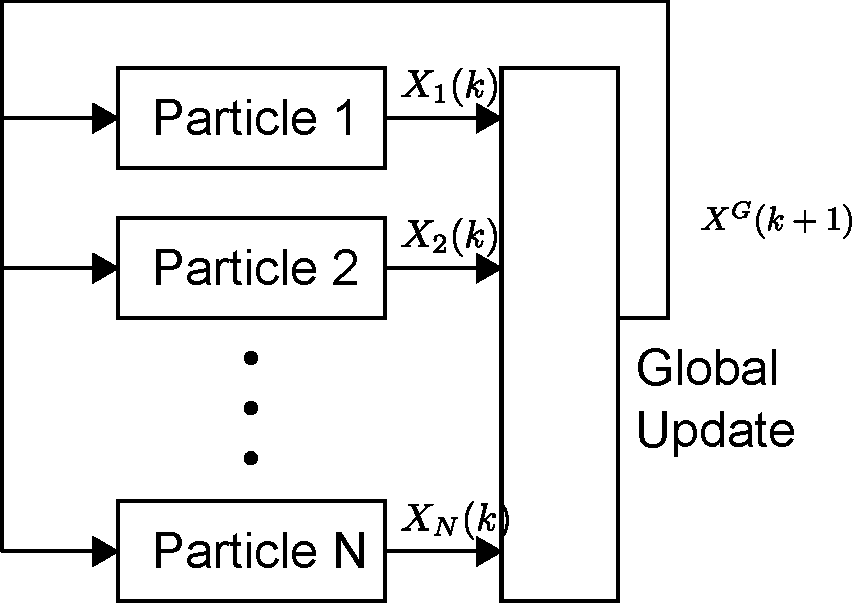
\includegraphics[width=\textwidth]{fig/pso_sys_flow.pdf}
		\caption{System structure of Swarm.}
		\label{fig:sys:swarm}
	\end{subfigure}   
	\caption{System structure of PSO.}
	\label{fig:sys:pso}
\end{figure}

For the purpose of input-to-state stability analysis we decompose the PSO algorithm into components as shown in Figure \ref{fig:sys:particle}. 
This decomposition is comprised of cascaded components (the input update, followed by the position update) and the feedback of the historical state.
These two components are the 
\emph{input-update component} for the global best ($ x^{G}_{i}(k) $) and the personal best ($ x^{P}_{i}(k) $), and the 
\emph{position-update component} for particle position ($ x_{i}(k+1) $), which depends on the inputs $ x^{G}_{i}(k) $ and $ x^{P}_{i}(k) $ as well as the previous position $ x_{i}(k) $.

The properties of this system can be analyzed using the input-to-state stability of the position-update component and the input-update component. 
The input-to-state stability analysis of the position-update component supports the parameter selection for the balance between the exploration and exploitation in the PSO algorithm.
We provide the condition that guarantees that the position-update component is input-to-state stable as a theorem.
Let $ \phi^{sup}  = \phi^{G} + \phi^{P} $, we can have an input-to-state stable region in the parameter space as shown in Figure \ref{fig:paramSpace}.

\begin{figure}[htbp]
	\centering
	\begin{subfigure}[t]{0.4\linewidth}
		\centering
		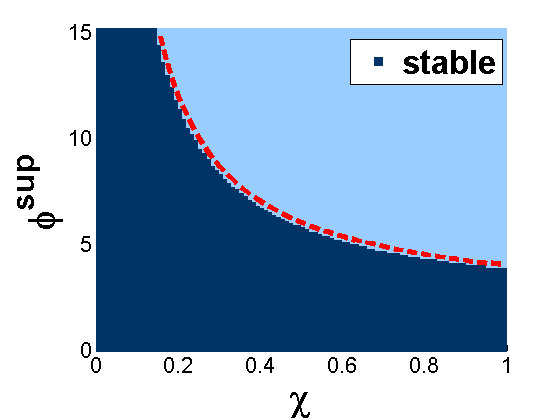
\includegraphics[width=\textwidth]{./fig/param2.png}
		\caption{Parameter space.}
		\label{fig:paramSpace}
	\end{subfigure}  
	%\\
	\begin{subfigure}[t]{0.55\linewidth}
		\centering
		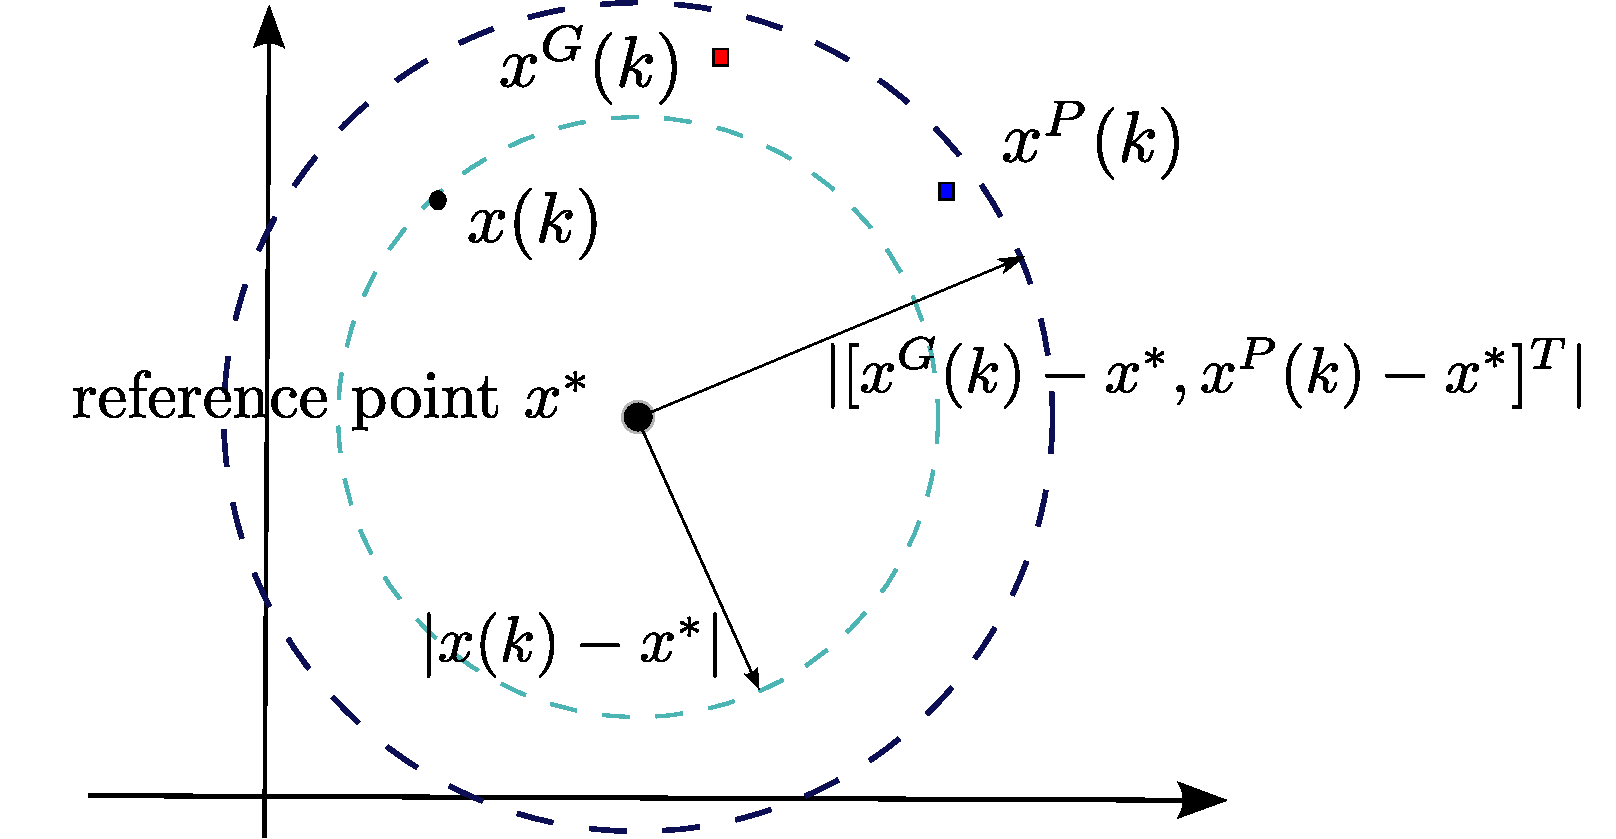
\includegraphics[width=\textwidth]{./fig/boundary}
		\caption{A bound on a particle's position by a reference point $ x^{*} $ from Equation %\eqref{eq:state_bound:conv}.
		The ratio of two radii indicates $ \gamma $..}
		\label{fig:boundary}
	\end{subfigure}   
	\caption{Parameter space and the boundary of a particle.}
	\label{fig:particle:param_bound}
\end{figure}

Given an input-to-state stable position-update component, we will see that the convergence of $ x_{i}(k) $ depends on bounds on $ x^{G}_{i}(k) $ and $ x^{P}_{i}(k) $.
Figure \ref{fig:boundary} illustrates a boundary on the particle motion, which indicates the exploring capability and exploitation property of one particle.
As in the Figure \ref{fig:sys:swarm}, the particles in the swarm form a networked feedback structure.
Integrating the input-to-state stability of each component in the swarm helps us understand the convergence of the swarm.
This helps us to analyze the capability of optimal search of the PSO in different fitness landscapes with different parameter selections.


%%%%%%%%%%%%%%%%%%%%%%%%%%%%%%%%%%%%%%%%%%%%%%%%%%%%%%%%%%%%%%%%%%%%%%%%%%%%%%%
\section{Dissertation Schedule}
% about 1/2 page
% specifying dates for completion of major milestones, including potential
% papers and their submission dates

\begin{itemize}
\item Conference Paper: Toward Task-Based Mental Models of Human-Robot Teaming: A Bayesian Approach. (HCII 2013, July 2013)
\item Conference Paper: Supporting Task-oriented Collaboration in Human-Robot Teams using Semantic-based Path Planning. (DSS 2014, June 2014)
\item Conference Paper: Path Planning with a Human
Path Constraint. (IEEE SMC 2014, October 2014)
\item Conference Paper: Input-to-State Stability Analysis on Particle Swarm Optimization. (GECCO 2015, July 2015)
\item Conference Paper: MORRF$^{*}$ : Sampling-based Multi-Objective Motion Planning. (IJCAI 2015, July 2015)
\item Journal Paper: Understanding the Particle Swarm Optimization by component decomposition. (TEVC, Submitted by June 2015)
\item Conference Paper: Homotopy-Aware RRT$^{*}$ : Toward Human-Robot Topological Path-Planning. (AAAI 2016, Submitted by September 2016)
\item Submission of the dissertation to advisor (March 2016)
\item Journal Paper: Sampling-based Multi-Objective Path Planning (Submitted by September 2016)
\item Conference Paper: Robotic environment learning with human instructions (IJCAI 2016, Submitted by February 2016)
\item Submission of the dissertation to committee members (April 2016)
\item Dissertation Defense (June 2016)
\item Journal Paper: Finding the optimal path planning with different homotopy classes (Submitted by April 2016)
\end{itemize}

%%%%%%%%%%%%%%%%%%%%%%%%%%%%%%%%%%%%%%%%%%%%%%%%%%%%%%%%%%%%%%%%%%%%%%%%%%%%%%%
% Change these to reflect the bibliography style and bibtex database file you want to use
\bibliographystyle{plain}
\bibliography{proposal_ref}

\end{document}
